One lasting scientific legacy of the {\it Hubble Space Telescope
(HST)} is the discovery of massive black holes at the centers of 
a substantial fraction of galaxies, confirming the longstanding theory of the ``central
engines'' of quasars.  One of the major surprises from the {\it
Hubble} was the discovery of a strong correlation between black hole mass and
host galaxy properties.\footnote{Assessment of Options for Extending
the Life of the Hubble Space Telescope: Final Report (2005);
https://www.nap.edu/read/11169/chapter/5).}  This connection, causal
or otherwise, may provide crucial clues to how and why these black
holes formed and how their host galaxies evolved. {\it As of the
launch of the James Webb Space Telescope (JWST), the question of how
black holes affect their host galaxies is one of the outstanding
questions in astrophysics.}

\smallskip \smallskip
\noindent
Observational and theoretical work now suggests that active galaxies
and black holes are potentially linked to both the triggering, and
``quenching'', of massive star formation. The link between massive
galaxies and the central super-massive black holes (SMBHs) that appear 
ubiquitous is vital to the understanding of
galaxy formation and evolution, and significant observational and
theoretical effort has been invested in trying to measure and
understand the physics involved in these systems.  The two
main energy sources available to a galaxy are nuclear fusion in stars
and gravitational accretion onto compact objects, and we still do not
fully understand the interaction of an active galactic nuclei and the
star formation properties of their host galaxies. % {\it especially at
%the epoch of maximal cosmic SFR and quasar activity, redshifts $z\sim1-3$.}

\smallskip \smallskip
\noindent
The ``quenching'' of galaxy-wide star formation is supposedly driven
by `` AGN feedback'', where the AGN heats the surrounding gas
corona, offsetting cooling losses and disrupting the gas inflow. This
feedback manifests itself as high-velocity outflows from the
AGN.  However, {\it direct observational evidence} for AGN
feedback is conspicuous by its absence. This statement is especially true at
high-$z$, e.g. $z=2-3$, at the height of the Quasar Epoch.  We have
identified the best candidates that would possess quasar
feedback in action, in situ at high-redshift. These are the
``Extremely Red Quasars'' identified via their WISE W3/4 colors.  As
such, these mJy luminous AGN {\it are ideal targets for JWST
MIRI}.


\section*{The Extremely Red Quasar Population} 
{\it Extremely Red Quasars (ERQs) are a unique obscured quasar
population with extreme physical conditions related to powerful
outflows across the line-forming regions. These sources are the
signposts of the most extreme form of quasar feedback at the peak
epoch of galaxy formation, and may represent an active ``blow-out''
phase of quasar evolution.}

\smallskip
\smallskip
\noindent
By matching the quasar catalogues of the Sloan Digital Sky Survey
(SDSS) and the Baryon Oscillation Spectroscopic Survey (BOSS) to the
Wide-Field Infrared Survey Explorer (WISE), Ross et al. (2015)
discovered quasars with extremely red infrared-to-optical colors:
$r_{\rm AB}-W4_{\rm Vega}>14$ mag, i.e., $F_\nu({\rm 22\mu
m})/F_\nu(r) \gtrsim 1000$; see Figure 1. These objects have infrared
luminosities $\sim 10^{47}$ erg s$^{-1}$, and this initial study
returned a heterogeneous population, spanning a wide redshift
range $0.28 < z < 4.36$.

\smallskip
\smallskip
\noindent
Hamann et al. (2017) refined the selection of the ERQs, homing the
definition based on additional analysis and common properties, and 
found several more objects in this new scheme. The ERQs have a
suite of peculiar emission-line properties including large rest
equivalent widths (REWs), unusual ``wingless'' line profiles, large
\nv /\lya , \nv /\civ , \siiv /\civ\ and other flux ratios, and very
broad and blueshifted [\oiii ] \lam 5007 (e.g., Figure~1, top right).

\hspace{-7.5cm}
\begin{figure}[h]
  \begin{center}
    \hspace{-0.5cm}
    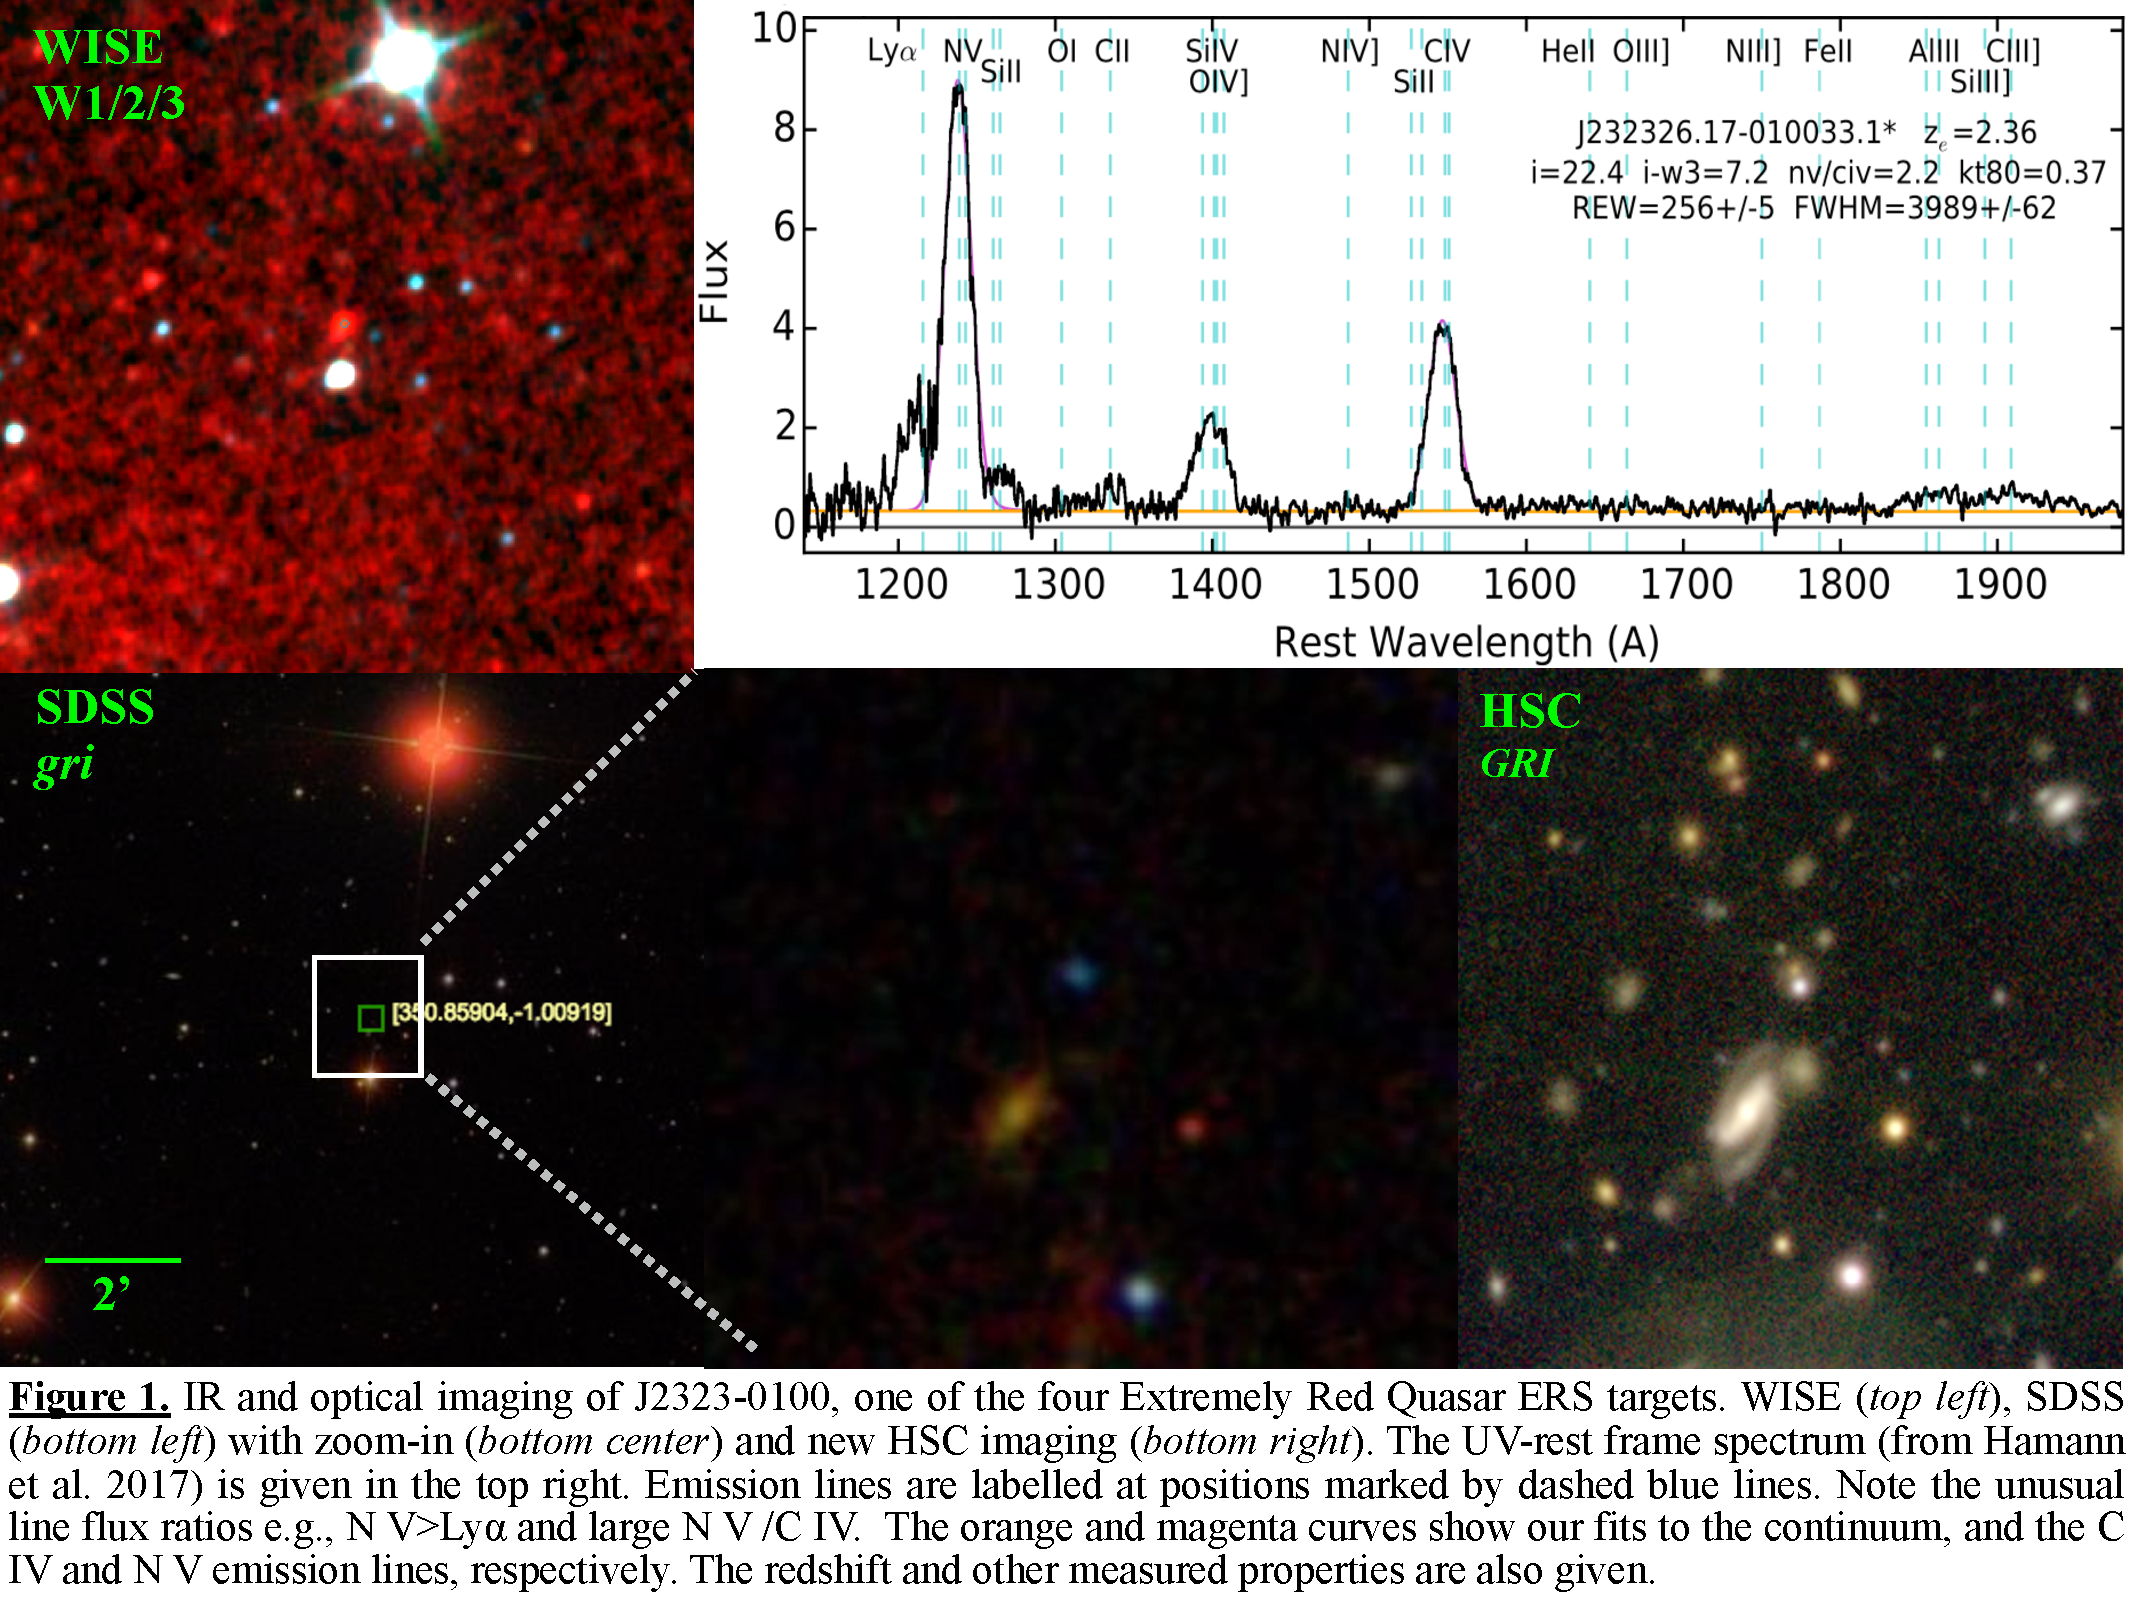
\includegraphics[height=12.0cm,width=16.0cm]{../Figures/WISE_SDSSzoomHSC_ERQ-image_v2.pdf}
    \vspace{-10pt}
    \vspace{-14pt}
    \label{figtest-fig}
  \end{center}
\end{figure}

\setcounter{figure}{1}
\hspace{-2.5cm}
\begin{figure}[h]
  \begin{center}
    \hspace{-0.5cm}
    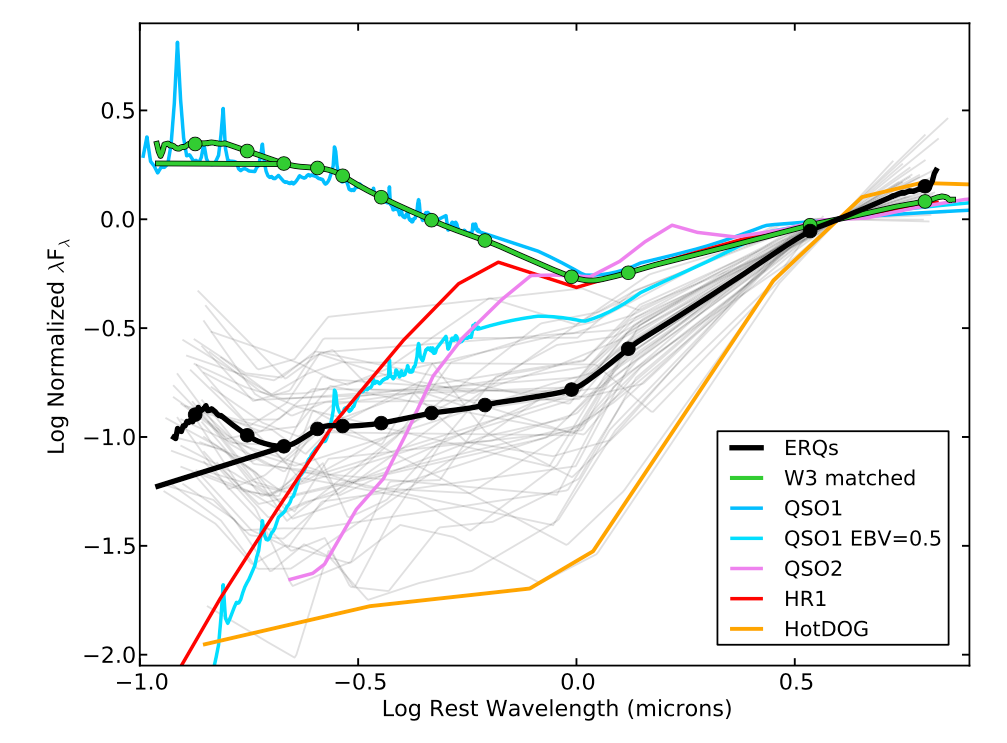
\includegraphics[height=7.0cm,width=7.0cm]{../Figures/Hamann2017_Fig16_SEDs.png}
    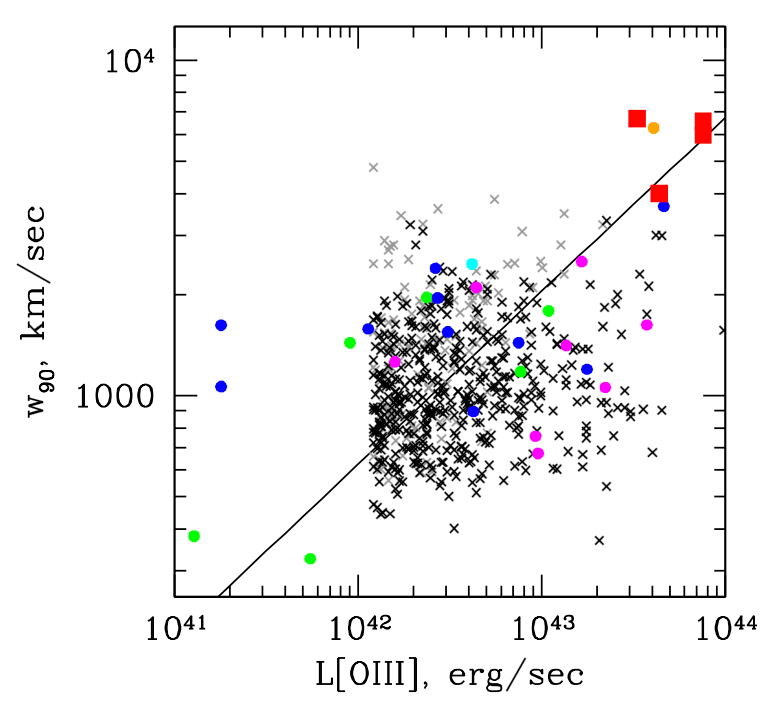
\includegraphics[height=7.1cm,width=7.4cm]{../Figures/Zakamska_2016_Fig9.png}
    \vspace{-10pt}
    \caption{
      % \small
      %\footnotesize
      \scriptsize
      % \tiny
      {\it (Left)} From Hamann et al., 2017, the normalized median
      SEDs for Type 1 non-BALs in the core ERQ sample (black curve) plus
      blue quasars matched to the core ERQs in W3 magnitude (green curve).
      The Type 1 quasar template with and without reddening equal to $E(B −
      V) = 0.5$ (light blue, `QSO1', from Polletta et al. 2007), a typical
      Type 2 quasar from Mateos et al. (2013; `QSO2', purple), a typical
      heavily reddened Type 1 quasar from Banerji et al. (2013; `HR1'), and
      a typical HotDOG from Tsai et al. (2015). The light grey curves are
      SEDs of individual core ERQs.
      %%
      {\it (Right)} \oiii\ kinematics as a function of luminosities
      for our four targets, red squares, with other quasar populations are
      shown by black points and various colored symbols.  At these extreme
      velocities, the gas cannot be confined by any realistic galaxy
      potential and is thus likely to escape from the galaxy; these objects
      are likely signposts of the extreme ‘blow-out’ phase of quasar
      feedback observed at the peak epoch of galaxy formation.
    }
    \vspace{-14pt}
    \label{fig:ERQ_SED}
  \end{center}
\end{figure}

\vspace{-22pt}
%\smallskip
%\smallskip
\noindent
Our team has identified a core sample of 97 ERQs with nearly uniform
peculiar properties selected via \imw\ $\ge 4.6$ (AB) and REW(\civ )
$\ge$ 100 \AA\ at redshifts 2.0--3.4.  The core ERQs have median
luminosity $\left<\log L ({\rm ergs/s})\right> \sim 47.1$, sky density
0.010 deg$^{-2}$, surprisingly flat/blue UV spectra given their red
UV-to-mid-IR colors, and common outflow signatures including BALs or
BAL-like features and large \civ\ emission-line blueshifts. Their
SEDs (see Figure~\ref{fig:ERQ_SED}) and line properties are
inconsistent with normal quasars behind a dust reddening
screen. Patchy obscuration by small dusty clouds could produce the
observed UV extinctions without substantial UV reddening.


\smallskip
\smallskip
\noindent
Further observations by our team with VLT/XShooter measured rest-frame
optical spectra of four of the $z\sim 2.5$ ERQs (Zakamska et al. 2016) 
which revealed very broad (FWHM = 2600-5000 km
s$^{-1}$), strongly blue-shifted (by up to 1500 km s$^{-1}$)
\oiii\ $\lambda$5007\AA\ emission lines in these objects. In a large
sample of type 2 and red quasars, \oiii\ kinematics are positively
correlated with infrared luminosity, and the four objects in our
sample are on the extreme end both in \oiii\ kinematics and infrared
luminosity.
%%
As such, we estimate that at least 3\% of the bolometric luminosity in
these objects is being converted into the kinetic power of the
observed wind. Photo-ionization estimates suggest that the \oiii\ 
emission might be extended on a few kpc scales, which would suggest
that the extreme outflow is affecting the entire host galaxy of the
quasar.

%\smallskip
%\smallskip
%\noindent
%{\it Given the extreme nature of these objects, especially in the 
%kinematics,  what is the power source for the IR luminosity? 
%Is it young, hot stars in a starburst, or hot dust powered by the central AGN?
%Furthermore, how, if at all, is this IR emission connected to the
%conditions at large of the quasar and host galaxy?}


%% \medskip
%% \medskip
%% \smallskip
%% \smallskip
%% \noindent
%% {\bf \underline{MIR spectroscopy}:}
%% In order to quantify the main energy contribution in galaxies, one needs to differentiate objects powered by nuclear fusion in stars from objects powered by mass accretion onto supermassive black holes. MIR spectroscopy allows the detection of obscured AGN components even when the MIR is dominated by the host galaxy. Several classification diagrams have been developed to determine the AGN contribution to an observed spectrum based on certain spectral features, such as high ionisation emission lines like \nev, \neii and \oiv, the EW of PAH features and the strength of the silicate feature at 9.7 $\mu$m. A number of techniques have also been developed to model the observed MIR spectra and constrain the AGN and starburst contributions (see e.g. Schweitzer et al., 2008; Nardini et al., 2008; Deo et al., 2009; Feltre et al., 2013). 
%% [Ne V] 14.3, 24.2 μm 97.
%% [Ne II] 12.8 μm
%% [OIV] 26μm


\smallskip
\smallskip
\noindent
%{\bf \underline{Polycyclic Aromatic Hydrocarbons}:}
{\bf \underline{MIR spectroscopy and PAHs}:}
Polycyclic Aromatic Hydrocarbons (PAHs) are abundant, ubiquitous, and
a dominant force in the interstellar medium of galaxies (see e.g., for
a review).  Aromatic features are already a significant component of
dusty galaxy spectra as early as $z\approx2$.  and the infrared (IR) emission features at 3.3, 6.2, 7.7,
8.6, and 11.3 $\mu$m are generally attributed to IR fluorescence from
(mainly) far-ultraviolet (FUV) pumped large polycyclic aromatic
hydrocarbon (PAH) molecules. As such, these features trace the FUV
stellar flux and are thus a measure of star formation.  The
interstellar IR emission spectrum is incredibly rich and shows a
wealth of detail.  It is dominated by major emission features at 3.3,
6.2, 7.7, 8.6, 11.2, 12.7, and 16.4 $\mu$m.  In addition, there are
weaker features at 3.4, 3.5, 5.25, 5.75, 6.0, 6.9 and 7.5$\mu$m.  
{\it Given the redshift of our ERQs and
the MIRI wavelength coverage we will coverage $1.36 \leq \lambda_{\rm
emitted} \leq 8.6 \mu$m.}
In theory, we can detect the 3$\mu$m water-ice feature, 
and figure out where it is most prevalent in the quasar. 

\smallskip
\smallskip
\noindent
The mid-IR spectral region
also presents a suite of high-ionization lines: \snine\ at
1.252$\mu$m, \six\ at 1.430$\mu$m, \sixi\ at 1.932$\mu$m, \sivi\ at
1.962$\mu$m, \caviii\ at 2.321$\mu$m, \sivi\ at 2.483$\mu$m \siix\ at
3.935$\mu$m and \arii\ at 6.97$\mu$m.
% such as [Ne ii]12.8 μm, [Ne v]14.3 μm, [Ne iii]15.5 μm, [S iii]18.7 μm and 33.48 μm, [O iv]25.89 μm and [Si ii]34.8 μm (e.g
%% Note from Fred::
%% MIR emission lines like [NeII] and [NeV] are ..
%%
%% Also,  arXiv:astro-ph/0003457v1 
%% [NeV] 14.32um & 24.32um and [NeVI] 7.65um imply an A(V)>160 towards the NLR...
%% [NeIII]15.56um/[NeII]12.81um
%%
%%
However, most critically, we have access to the 
\nevi\ line at 7.65$\mu$m, which with an Ionization potential of 158 eV is much too high for stars.
 Critical density of  106 cm-3 and very low interstellar extinction
 Ratio to hydrogen recombination lines virtually independent of ionization parameter • 
{\bf The [Ne VI] 7.65 mm line can be used to measure the instantaneous luminosity of the central engine.}
Not readily confused with high mass X-ray binaries
%
The calibration should remain valid over the expected range of metallicity.

%\snine\ at 1.252$\mu$m, \six\ at 1.430$\mu$m, \sixi\ at 1.932$\mu$m, \sivi\ at
%1.962$\mu$m, \caviii\ at 2.321$\mu$m, \sivi\ at 2.483$\mu$m \siix\ at
%3.935$\mu$m and \arii\ at 6.97$\mu$m. 
% such as [Ne ii]12.8 μm, [Ne v]14.3 μm, [Ne iii]15.5 μm, [S iii]18.7 μm and 33.48 μm, [O iv]25.89 μm and [Si ii]34.8 μm (e.g

%With our first science goal being to detect PAH features, a second goal will be to measure the strengths of the MIR emission lines such as [NeII] and [NeV].  are mentioned only briefly at one point, so it’s not clear if they are an objective of this program. I think we need to say more about that because, if those lines are present, we'll measure them. We should at least mention some specific lines and wavelengths and their potential implications for the science. But then what’s really needed for both these lines and the PAHs are estimates of the feature strengths (probably scaling from local ULIRG/quasar observations)...

\smallskip
\smallskip
\noindent
{\it With the IFU spatial information, at medium resolution, we will be able to 
(i) map the PAH emission structure of the extremely red quasars and (ii) look 
for offsets in these emissions that could well be indicative of `AGN feedback.}

\smallskip
\smallskip
\noindent
{\bf \underline{Integral Field Unit Observations.}}
The ability for the MRS to obtain integral field unit spectroscopy
allows us to investigate the {\it spatial information} associated with
the high IR fluxes in the ERQs. The spatial distribution of the IR
will give direct clues to the power source of the IR emission.  The
IFU aspect of the Medium Resolution Spectrometer will allow
unprecendet detailed investigations of the both the central AGN IR
emission and any potentially extended emission in $z\approx2.5$
quasars.  As a null hyopthesis, we suggest that weak PAH emission will
be in the nuclear regions and strong(er) PAH emission in the extended
source. However, very recent studies with H$\alpha$ in of$z\sim2$
quasars suggest that narrow H$\alpha$ emission might be from a
spatially unresolved source.

\smallskip \smallskip
\noindent 
Our final primary science goal will be to examine the IR spectral
emission lines (PAH or high ionization) and place them in context with
the host galaxy by looking for emisson line offsets or extreme blends.
The kinematics of the \oiii\ $\lambda \lambda$4959,5007 \AA\ emission
lines are {\it known to extreme} in these objects, being very broad
(FWHM=2600-5000 km s$^{-1}$) and strongly blueshifted (by up to 1500
km s$^{-1}$; Figure 2, {\it right}). We also know that the \oiii\
kinematics are positively correlated with infrared luminosity.  Can we
place the PAH and AGN emission in the same consistent kinematic
structure?  Is there a spatial variaion of the kinematics of the IR
emission lines, and if so, is it consistent with a strong `AGN
feedback' phase?


\iffalse
 think this needs more development to get to the point of saying how we will interpret our observations. What will learn from different outcomes with strong/weak/absent PAH emission? We need to mention the alternative that the MIR could be from hot dust powered by the AGN. This scenario would yield weak PAHs, but I think it does imply low SFRs. This is not something I’ve worked on or thought about in any detail, but I think we should frame this as a question about what powers the MIR luminosities - hot stars in a starburst or the central AGN. That mean diving into the literature about PAH equivalent widths and how they’re interpreted in other sources across the ULIRG - quasar continuum, starting with the famous Genzel+98 diagrams but then more recent work… Another aspect of this is the spatial information. Maybe we will find weak PAHs in the nuclear regions and strong PAHs farther out. That seems likely. But then we should talk about the spatial resolution, spatial scales in kpc, compare that to the sizes measured for SMGs (they pretty compact, I think just a few kpc across). Etc.
\fi

%%\normalsize (default) \small \footnotesize \scriptsize \tiny
\footnotesize
\section*{Bibliography}
\vspace{-8pt}
Alaghband-Zadeh et al., 2016, MNRAS, 459, 999 $\bullet$
Alexander et al. 2005, Nature, 434, 738  $\bullet$
Alexander et al., 2008, AJ, 135, 1968	 $\bullet$
Alexander et al., 2010, MNRAS, 402, 2211 $\bullet$
Banerji et al., 2015, MNRAS, 447, 3368 $\bullet$
Banerji et al., 2017, MNRAS, 465, 4390 $\bullet$
Armus et al., 2007, ApJ, 656, 148 $\bullet$
Fabian, 2012, ARAA 50, 455 $\bullet$ 
Cano-Diaz et al., 2012, A\&A, 537, L8 $\bullet$  
Coppin et al., 2004, MNRAS, 354, 193 $\bullet$
Coppin et al., 2008, MNRAS, 389, 45 $\bullet$
Coppin et al., 2010, ApJ, 713, 503 $\bullet$
Cresci et al., 2015, ApJ, 799, 82 $\bullet$
Daddi et al., 2007, ApJ, 670, 173	$\bullet$
Fu et al., 2010, ApJ, 722, 653 	$\bullet$
Glikman et al., 2015, ApJ, 806, 218 $\bullet$
Hamann et al., 2017, MNRAS, 464, 3431 $\bullet$
Hernan-Caballero \& Hatziminaoglou, 2011, MNRAS, 414, 500	$\bullet$
Higdon et al., 2004, PASP, 116, 975 $\bullet$
Kormendy \& Ho, 2013, ARAA, 51, 511 $\bullet$
Heckman \& Best, 2014, ARAA, 52, 589  $\bullet$
Mampaso, Prieto \& Sánchez, Infrared Astronomy, 2004, ISBN  9780521548106 $\bullet$
Mullaney et al., 2011, MNRAS, 414, 1082  $\bullet$
Mullaney et al., 2012, MNRAS, 419, 95 $\bullet$
Peeters et al, 2004, ApJ, 613, 986 $\bullet$
Pope et al. 2008, ApJ, 675, 1171 $\bullet$
Ross et al., 2013, ApJ, 773, 14 $\bullet$
Ross et al., 2015, MNRAS, 453, 3932 $\bullet$
Sajina et al., 2007, ApJ, 664, 713 $\bullet$
Sajina et al., 2009, ApJ, 703, 270 $\bullet$
Spoon et al., 2007, ApJ, 654, L49 $\bullet$
Tielens, 2008, ARAA, 46, 289  $\bullet$
Veilleux et al., 2009, arXiv:0201118v1 ;$\bullet$

Yan et al., 2005, ApJ, 628, 604 $\bullet$
Yan et al, 2007, ApJ, 658, 778 $\bullet$
Yuan \& Narayan, 2014, ARAA, 52, 529 $\bullet$
Zakamska et al., 2016, MNRAS, 459, 3144 

\normalsize
\medskip \medskip \medskip \medskip
%\clearpage


